\documentclass{standalone}
\usepackage{tikz}
\usetikzlibrary{patterns, positioning}


\begin{document}
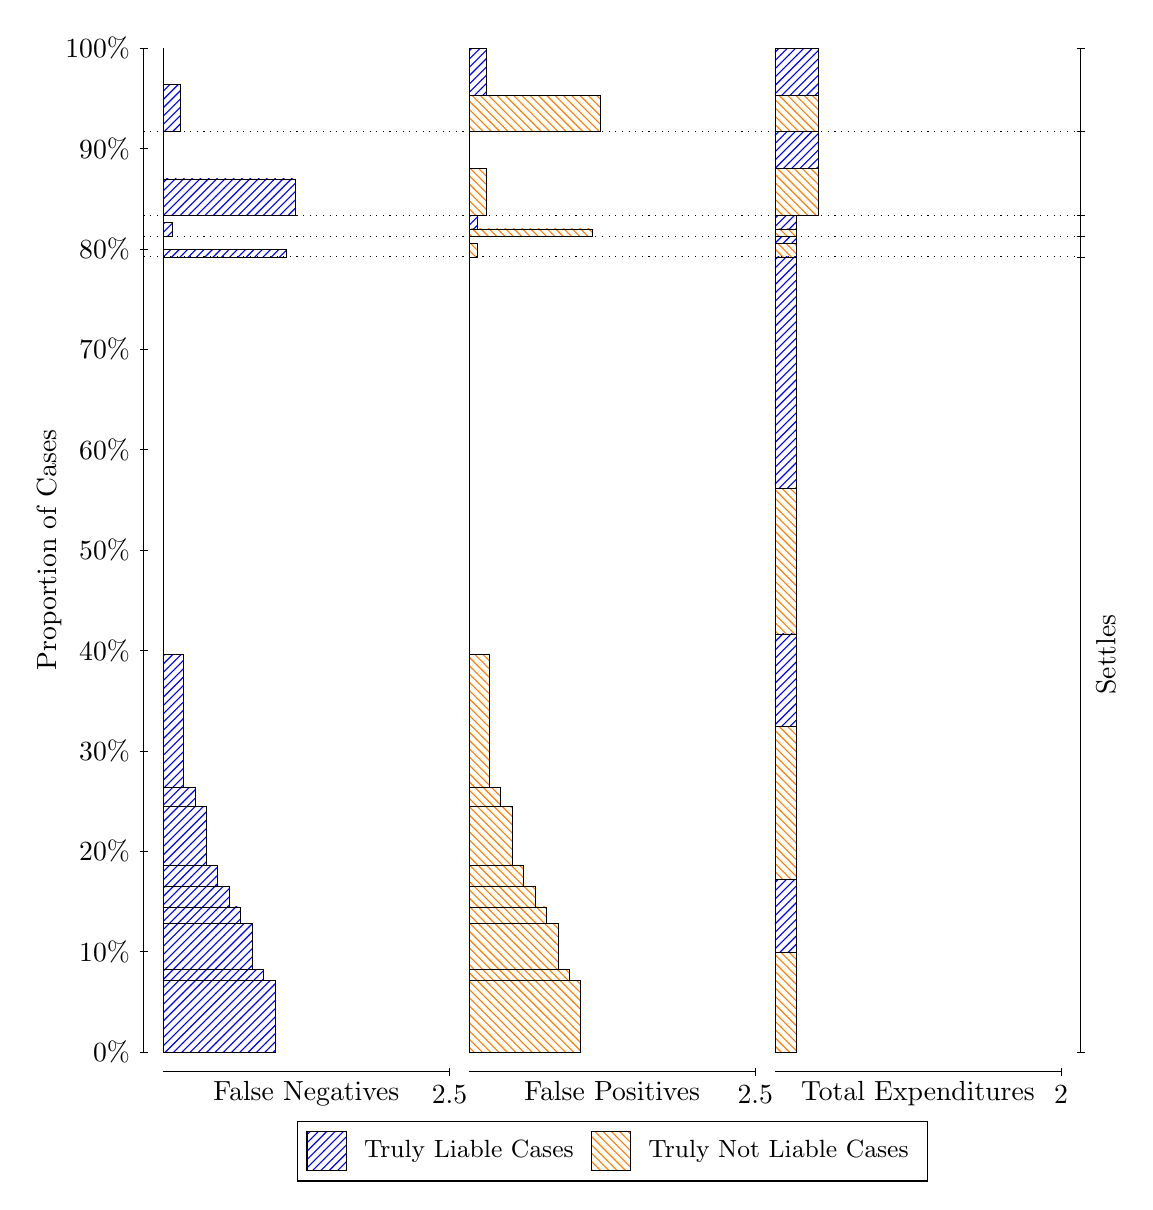
\begin{tikzpicture}
\draw[black, very thin] (1.5,1.75) -- (1.5,14.5);
\node[rotate=90, text=black, anchor=center] at (0.3, 8.125) {Proportion of Cases};
\draw[black, very thin] (1.45,1.75) -- (1.55,1.75);
\node[text=black, anchor=east] at (1.45, 1.75) {0\%};
\draw[black, very thin] (1.45,3.025) -- (1.55,3.025);
\node[text=black, anchor=east] at (1.45, 3.025) {10\%};
\draw[black, very thin] (1.45,4.3) -- (1.55,4.3);
\node[text=black, anchor=east] at (1.45, 4.3) {20\%};
\draw[black, very thin] (1.45,5.575) -- (1.55,5.575);
\node[text=black, anchor=east] at (1.45, 5.575) {30\%};
\draw[black, very thin] (1.45,6.85) -- (1.55,6.85);
\node[text=black, anchor=east] at (1.45, 6.85) {40\%};
\draw[black, very thin] (1.45,8.125) -- (1.55,8.125);
\node[text=black, anchor=east] at (1.45, 8.125) {50\%};
\draw[black, very thin] (1.45,9.4) -- (1.55,9.4);
\node[text=black, anchor=east] at (1.45, 9.4) {60\%};
\draw[black, very thin] (1.45,10.675) -- (1.55,10.675);
\node[text=black, anchor=east] at (1.45, 10.675) {70\%};
\draw[black, very thin] (1.45,11.95) -- (1.55,11.95);
\node[text=black, anchor=east] at (1.45, 11.95) {80\%};
\draw[black, very thin] (1.45,13.225) -- (1.55,13.225);
\node[text=black, anchor=east] at (1.45, 13.225) {90\%};
\draw[black, very thin] (1.45,14.5) -- (1.55,14.5);
\node[text=black, anchor=east] at (1.45, 14.5) {100\%};

\draw[black, very thin] (13.4,1.75) -- (13.4,14.5);
\draw[black, very thin] (13.35,1.75) -- (13.45,1.75);
\node[anchor=west] at (13.35, 1.75) {};
\draw[black, very thin] (13.35,11.848) -- (13.45,11.848);
\node[anchor=west] at (13.35, 11.848) {};
\draw[black, very thin] (13.35,12.112) -- (13.45,12.112);
\node[anchor=west] at (13.35, 12.112) {};
\draw[black, very thin] (13.35,12.375) -- (13.45,12.375);
\node[anchor=west] at (13.35, 12.375) {};
\draw[black, very thin] (13.35,13.438) -- (13.45,13.438);
\node[anchor=west] at (13.35, 13.438) {};
\draw[black, very thin] (13.35,14.5) -- (13.45,14.5);
\node[anchor=west] at (13.35, 14.5) {};

\draw[black, very thin, pattern color=blue, pattern=north east lines] (1.75,1.75) rectangle (3.167,2.6608);
\draw[black, very thin, pattern color=blue, pattern=north east lines] (1.75,2.6608) rectangle (3.0217,2.8);
\draw[black, very thin, pattern color=blue, pattern=north east lines] (1.75,2.8) rectangle (2.8763,3.383);
\draw[black, very thin, pattern color=blue, pattern=north east lines] (1.75,3.383) rectangle (2.731,3.5928);
\draw[black, very thin, pattern color=blue, pattern=north east lines] (1.75,3.5928) rectangle (2.5857,3.854);
\draw[black, very thin, pattern color=blue, pattern=north east lines] (1.75,3.854) rectangle (2.4403,4.1193);
\draw[black, very thin, pattern color=blue, pattern=north east lines] (1.75,4.1193) rectangle (2.295,4.8703);
\draw[black, very thin, pattern color=blue, pattern=north east lines] (1.75,4.8703) rectangle (2.1497,5.1151);
\draw[black, very thin, pattern color=blue, pattern=north east lines] (1.75,5.1151) rectangle (2.0043,6.799);
\draw[black, very thin, pattern color=orange, pattern=north west lines] (1.75,6.799) rectangle (1.75,11.848);
\draw[black, very thin, pattern color=blue, pattern=north east lines] (1.75,11.848) rectangle (3.3123,11.94);
\draw[black, very thin, pattern color=orange, pattern=north west lines] (1.75,11.94) rectangle (1.75,12.112);
\draw[black, very thin, pattern color=blue, pattern=north east lines] (1.75,12.112) rectangle (1.859,12.283);
\draw[black, very thin, pattern color=orange, pattern=north west lines] (1.75,12.283) rectangle (1.75,12.375);
\draw[black, very thin, pattern color=blue, pattern=north east lines] (1.75,12.375) rectangle (3.4213,12.838);
\draw[black, very thin, pattern color=orange, pattern=north west lines] (1.75,12.838) rectangle (1.75,13.438);
\draw[black, very thin, pattern color=blue, pattern=north east lines] (1.75,13.438) rectangle (1.968,14.037);
\draw[black, very thin, pattern color=orange, pattern=north west lines] (1.75,14.037) rectangle (1.75,14.5);
\draw[black, very thin, pattern color=orange, pattern=north west lines] (5.6333,1.75) rectangle (7.0503,2.6607);
\draw[black, very thin, pattern color=orange, pattern=north west lines] (5.6333,2.6607) rectangle (6.905,2.7999);
\draw[black, very thin, pattern color=orange, pattern=north west lines] (5.6333,2.7999) rectangle (6.7597,3.3829);
\draw[black, very thin, pattern color=orange, pattern=north west lines] (5.6333,3.3829) rectangle (6.6143,3.5928);
\draw[black, very thin, pattern color=orange, pattern=north west lines] (5.6333,3.5928) rectangle (6.469,3.854);
\draw[black, very thin, pattern color=orange, pattern=north west lines] (5.6333,3.854) rectangle (6.3237,4.1192);
\draw[black, very thin, pattern color=orange, pattern=north west lines] (5.6333,4.1192) rectangle (6.1783,4.8703);
\draw[black, very thin, pattern color=orange, pattern=north west lines] (5.6333,4.8703) rectangle (6.033,5.1151);
\draw[black, very thin, pattern color=orange, pattern=north west lines] (5.6333,5.1151) rectangle (5.8877,6.799);
\draw[black, very thin, pattern color=blue, pattern=north east lines] (5.6333,6.799) rectangle (5.6333,11.848);
\draw[black, very thin, pattern color=orange, pattern=north west lines] (5.6333,11.848) rectangle (5.7423,12.019);
\draw[black, very thin, pattern color=blue, pattern=north east lines] (5.6333,12.019) rectangle (5.6333,12.112);
\draw[black, very thin, pattern color=orange, pattern=north west lines] (5.6333,12.112) rectangle (7.1957,12.204);
\draw[black, very thin, pattern color=blue, pattern=north east lines] (5.6333,12.204) rectangle (5.7423,12.375);
\draw[black, very thin, pattern color=orange, pattern=north west lines] (5.6333,12.375) rectangle (5.8513,12.975);
\draw[black, very thin, pattern color=blue, pattern=north east lines] (5.6333,12.975) rectangle (5.6333,13.438);
\draw[black, very thin, pattern color=orange, pattern=north west lines] (5.6333,13.438) rectangle (7.3047,13.901);
\draw[black, very thin, pattern color=blue, pattern=north east lines] (5.6333,13.901) rectangle (5.8513,14.5);
\draw[black, very thin, pattern color=orange, pattern=north west lines] (9.5167,1.75) rectangle (9.7892,3.0111);
\draw[black, very thin, pattern color=blue, pattern=north east lines] (9.5167,3.0111) rectangle (9.7892,3.9432);
\draw[black, very thin, pattern color=orange, pattern=north west lines] (9.5167,3.9432) rectangle (9.7892,5.8883);
\draw[black, very thin, pattern color=blue, pattern=north east lines] (9.5167,5.8883) rectangle (9.7892,7.0603);
\draw[black, very thin, pattern color=orange, pattern=north west lines] (9.5167,7.0603) rectangle (9.7892,8.903);
\draw[black, very thin, pattern color=blue, pattern=north east lines] (9.5167,8.903) rectangle (9.7892,11.848);
\draw[black, very thin, pattern color=orange, pattern=north west lines] (9.5167,11.848) rectangle (9.7892,12.019);
\draw[black, very thin, pattern color=blue, pattern=north east lines] (9.5167,12.019) rectangle (9.7892,12.112);
\draw[black, very thin, pattern color=orange, pattern=north west lines] (9.5167,12.112) rectangle (9.7892,12.204);
\draw[black, very thin, pattern color=blue, pattern=north east lines] (9.5167,12.204) rectangle (9.7892,12.375);
\draw[black, very thin, pattern color=orange, pattern=north west lines] (9.5167,12.375) rectangle (10.062,12.975);
\draw[black, very thin, pattern color=blue, pattern=north east lines] (9.5167,12.975) rectangle (10.062,13.438);
\draw[black, very thin, pattern color=orange, pattern=north west lines] (9.5167,13.438) rectangle (10.062,13.901);
\draw[black, very thin, pattern color=blue, pattern=north east lines] (9.5167,13.901) rectangle (10.062,14.5);
\draw[black, dotted] (1.5,11.848) -- (13.4,11.848);
\draw[black, dotted] (1.5,12.112) -- (13.4,12.112);
\draw[black, dotted] (1.5,12.375) -- (13.4,12.375);
\draw[black, dotted] (1.5,13.438) -- (13.4,13.438);
\draw[black, very thin] (1.75,1.5) -- (5.3833,1.5);
\node[text=black, anchor=north] at (3.5667, 1.5) {False Negatives};
\draw[black, very thin] (5.3833,1.45) -- (5.3833,1.55);
\node[text=black, anchor=north] at (5.3833, 1.45) {2.5};

\draw[black, very thin] (5.6333,1.5) -- (9.2667,1.5);
\node[text=black, anchor=north] at (7.45, 1.5) {False Positives};
\draw[black, very thin] (9.2667,1.45) -- (9.2667,1.55);
\node[text=black, anchor=north] at (9.2667, 1.45) {2.5};

\draw[black, very thin] (9.5167,1.5) -- (13.15,1.5);
\node[text=black, anchor=north] at (11.333, 1.5) {Total Expenditures};
\draw[black, very thin] (13.15,1.45) -- (13.15,1.55);
\node[text=black, anchor=north] at (13.15, 1.45) {2};

\node[text=black, centered, rotate=90] at (13.72, 6.799) {Settles};





\draw (7.449999999999999,1.5) node[draw=none] (baseCoordinate) {};
\begin{scope}[align=center]
        \matrix[scale=0.5, draw=black, below=0.5cm of baseCoordinate, nodes={draw}, column sep=0.1cm]{
            \node[rectangle, draw, minimum width=0.5cm, minimum height=0.5cm, pattern color=blue, pattern=north east lines] {}; &
            \node[draw=none, font=\small, text=black] (B) {Truly Liable Cases}; &
            \node[rectangle, draw, minimum width=0.5cm, minimum height=0.5cm, pattern color=orange, pattern=north west lines] {}; &
            \node[draw=none, font=\small, text=black] (B) {Truly Not Liable Cases}; \\
            };
\end{scope}

\end{tikzpicture}
\end{document}